% Chapter 7

\begin{savequote}[\quotewidth]

\qauthor{Shark}
\end{savequote}

\chapter{The determination of FAMEs and PAHs in diesel fuel by SFC×GC.} % Main chapter title
\label{Chapter7} % For referencing this chapter elsewhere, use \ref{Chapter7}

\section{Introduction}

In South Africa the quality of biodiesel is regulated by the technical standard
SANS 1935, and petrodiesel by SANS 342. There is a considerable overlap in the
requirements of the two, as discussed in Section \ref{sec:Comparison} and
illustrated in Figure \ref{fig:Venn}. Two of the requirements of SANS 342 that
do not overlap with SANS 1935 are the allowed amounts of polycyclic aromatic
hydrocarbons (PAHs) and fatty acid methyl esters (FAMEs). This chapter's
discussion introduces the application of SFC×GC to these determinations.

\subsection{FAMEs in diesel}

Biodiesel can be blended in all proportions with diesel obtained from petroleum
(\keyword{petrodiesel}). To reduce the carbon footprint of diesel fuel,
legislators are encouraging the use of blended fuels. In South Africa standard
grades of diesel may contain up to \SI{5}{\percent} volume fraction biodiesel,
and higher fractions of FAMEs are allowed as different grades. Manufacturers
might also add biodiesel to their fuel formulations to present improve
properties such as lubricity \autocite{Knothe2005}, or for its ability to reduce
engine emissions \autocite{Wattrus2016}.

The test methods for FAMEs in standard diesel prescribed by SANS 342 are EN
14078, ASTM D7806 and ASTM D7371. These are all infrared absorption methods. The
first two method measures the absorption of infrared radiation at
\SI{1745}{\per\centi\metre} (\SI{5.4}{\micro\metre}) in an absorption cell with
a path length of \SI{0.5}{\milli\metre}. A Beer's law calibration method is
used. The method prescribed by ASTM D7371 specifies an \keyword{attenuated total
reflection} (ATR) optical interface combined with \keyword{partial least squares
calibration}, which simplifies sample handling but complicates calibration. Both
these methods makes some assumptions about the sample, and the methods may
suffer from inaccuracy if those assumptions do not hold \autocite{Pinho2014}.

\subsection{PAHs in diesel} 

Polycyclic aromatic hydrocarbons (PAHs) are noxious pollutants and are therefore
regulated when possible. The primary source of PAHs in the environment is
combustion, of which a portion is in internal-combustion engines. PAHs are also
abundant in fossil fuels, including diesel, and might escape from diesel during
normal operations or in accidents. Primarily, however, the higher the proportion
of aromatic compounds in diesel fuel, the higher the PAH emissions of the engine
it fuels. These higher emissions are ascribed to the poorer combustion of fuels
containing higher amounts of aromatics. By limiting the amount of PAHs in diesel
regulators aim to reduce the exposure of the population to the harm of PAHs.

SANS 342 describes two classes of diesel fuel, CF1 and CF2, named after the
Department of Energy's Cleaner Fuels programme. For CF1 the standard does not
include a requirement for PAHs, but for CF2 an upper limit of \SI{8}{\percent}
mass fraction is prescribed. At the time of writing the implementation date of
the CF2 standard had been indefinitely postponed. 

The test methods for determining the amount of PAHs in diesel prescribed by SANS
342 are IP 391, ASTM D2425, EN 12916. In case of dispute EN 12916 is the referee
method. IP 391 and  EN 12916 are HPLC methods with \keyword{refractive index}
detection. ASTM D2425, although entitled ``Standard Test Method for Hydrocarbon
Types in Middle Distillates by Mass Spectrometry'' requires the chromatographic
separation of the aromatics from the saturates by chromatography before the MS
measurement. All these methods allow for the presence of FAMEs in diesel.
Although these methods undoubtedly provide reliable results when applied
intelligently, quantitation by refractive index and mass spectrometric detection
have their problems, which have been reviewed in detail \autocite{Kaminski2005}.
As an example of one of the challenges for RI detection, there is no correlation
between the refractive index of a compound and its chemical structure. Therefore
successful quantitation depends on the precise determination of response
factors. But in a mixture of petrochemicals from different feedstocks the
compounds and their relative quantities are unknown, so the physical meaning of
the determined peak areas is unclear.

Although not specified by SANS 342, ASTM D5186 \autocite{ASTMD5186} is an
SFC-FID method for determining the amount and type of aromatic compounds. In
principle it is similar to the prescribed HPLC methods, with three key
differences: it uses neat carbon dioxide at high pressure as a mobile phase, it
uses bare silica as a stationary phase, and it uses flame ionization as a
detector (FID). As discussed in Section \ref{sec:FID}, the FID has an
unsurpassed dynamic range and responds to the primarily to the number of carbon
atoms in the analyte, which means that its signal reflects the mass of the
analyte. This makes it a reliable and robust detector that excels at
quantitation.

\subsection{SFC×GC of petrodiesel/biodiesel blends}

The simplicity of coupling GC to SFC has been recognized and used for the
detailed analysis of hydrocarbon groups in diesel \autocite{Pal1998}.

The elution properties of aromatic hydrocarbons on SFC are different from that
of FAMEs. Being polar oxygenates, the FAMEs have a much higher retention than
the aromatic compounds, and the two classes elute completely separately. But,
just as the aromatic hydrocarbon compounds elute in order of their number of
rings, the FAMEs elute in order of their number of double bonds
\autocite{Smith2001}.

Comprehensively coupling GC to separate fractions of the SFC eluate on a second
dimension will then yield further information that correlates with the molecular
mass of the compounds.

\todo{k-primes}

\section{Experimental}

\subsection{Samples} 

A sample was prepared by blending \SI{7}{\percent} of biodiesel from canola
(labelled "rapeseed methyl ester" (RME)) with a commercial low-sulfur diesel.
(\SI{7}{\percent} was chosen to reflect the amount allowed by EN 590, the
European equivalent to EN 342). In a GC×GC-MS analysis the relative percentages
of total ion intensity for different classes of compounds were
\SI{68.19}{\percent} alkanes, \SI{18.10}{\percent} alkenes, \SI{13.69}{\percent}
aromatics and \SI{0.01}{\percent} oxygenates \autocite{Smit2015}.

To determine the relative retention times of aromatic compounds with different
numbers of rings, known amounts of a selection of aromatic compounds were added
(\keyword{spiked}) to a neat sample of the low-sulfur diesel. The retention
times of these compounds will give an indication of how the structure of an
aromatic compound influences its retention time, which will guide the 2D
chromatographic pattern interpretation. The selected compounds and their amounts
used in the spike are listed in Table \ref{tab:Aromatics}.


\begin{table}
\caption{Aromatic compounds added to a \SI{1.2819}{\gram} low sulfur diesel sample}
	\label{tab:Aromatics}
	\centering
	\renewcommand{\arraystretch}{2}%
	\begin{tabular}{|c|c|c|c|}
	\hline
	Structure & name & boiling point (°C) & mass (mg)\\
	\hline
	\raisebox{-.5\height}{\rule{0pt}{13mm}}\raisebox{-.5\height}{
\includegraphics{Figures/Aromatics/cumene.pdf}} & \text{cumene} & 153.\text{${}^{\circ}$C} & 8.4 \\
 	\hline	 
 	\raisebox{-.5\height}{\rule{0pt}{13mm}}\raisebox{-.5\height}{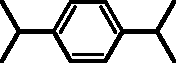
\includegraphics{Figures/Aromatics/diisopropylbenzene.pdf}} & \text{1,4-diisopropylbenzene} & 210.\text{${}^{\circ}$C} & 9.3 \\
 	\hline
 	\raisebox{-.5\height}{\rule{0pt}{18mm}}\raisebox{-.5\height}{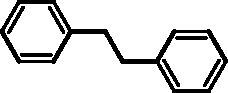
\includegraphics{Figures/Aromatics/bibenzyl.pdf} }& \text{bibenzyl} & 284.\text{${}^{\circ}$C} & 14.2 \\
 	\hline
 	\raisebox{-.5\height}{\rule{0pt}{15mm}}\raisebox{-.5\height}{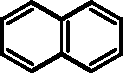
\includegraphics{Figures/Aromatics/naphthalene.pdf}} & \text{naphthalene} & 218.\text{${}^{\circ}$C} & 8.3 \\
 	\hline
 	\raisebox{-.5\height}{\rule{0pt}{15mm}}\raisebox{-.5\height}{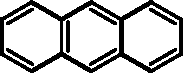
\includegraphics{Figures/Aromatics/anthracene.pdf} }& \text{anthracene} & 340.\text{${}^{\circ}$C} & 7.1 \\
 	\hline
 	\raisebox{-.5\height}{\rule{0pt}{22mm}}\raisebox{-.5\height}{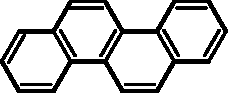
\includegraphics{Figures/Aromatics/chrysene.pdf}} & \text{chrysene} & 448.\text{${}^{\circ}$C} & 3.2 \\
 	\hline
 	\raisebox{-.5\height}{\rule{0pt}{23mm}}\raisebox{-.5\height}{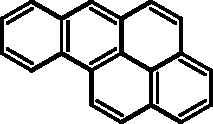
\includegraphics{Figures/Aromatics/benzo[a]pyrene.pdf}}& \text{benzo[a]pyrene} & 495.\text{${}^{\circ}$C} & 3.1 \\
 	\hline
\end{tabular}
\end{table}

\subsection{SFC}

The injection system described in Section \ref{sec:SFCInjection} was used to
inject a \SI{0.5}{\micro\litre} volume of the undiluted \SI{7}{\percent} blend
and the spiked sample. The SFC used neat carbon dioxide at \SI{200}{\bar} inlet
pressure as mobile phase. The column consisted of five HPLC bare silica columns
(\SI{150}{\milli\metre} $\times$ \SI{4.6}{\milli\metre}, 3 $\mu$m particles)
(Restek, Pinnacle DB Silica) connected in series.

\subsection{Modulation}

For the aromatic portion of the chromatogram SFC eluate fractions of
\SI{3}{\second} were collected on the GC column cooled to a temperature of
\SI{-20}{\celsius} or below. The inlet vent was held closed for \SI{3}{\second}
after the the SFC stop valve closed to allow the last of the eluted fraction to
be swept onto the column, and then opened for \SI{1}{\second} to release excess
pressure.

For the FAMEs portion of the chromatogram the same trapping temperature was
used, but the modulation period was increased to \SI{10}{\second}. This longer
trapping period causes a higher increase in inlet pressure by the eluting carbon
dioxide, which required a vent time of \SI{3}{\second} to release the excess
pressure.

\subsection{GC}

The column used in the fast gas chromatograph was an DB-5MS column from J\&W
Scientific Inc, which has a stationary phase comprised of \SI{5}{\percent}
diphenyl, \SI{95}{\percent} di\-meth\-yl\-poly\-si\-lox\-ane. It was \SI{1}{\metre} long,
with an internal diameter of \SI{0.25}{\milli\metre}. The thickness of the
stationary phase was \SI{0.25}{\micro\metre}, and had an operational temperature
range of \SI{-60}{\celsius} to \SI{325}{\celsius} for isothermal elution, or up
to \SI{350}{\celsius} when using temperature programming.

For every fast GC run the temperature was ramped from \SI{-30}{\celsius} at a
rate of \SI{8000}{\celsius\per\minute} to \SI{25}{\celsius}, and from there to
\SI{350}{\celsius} at a rate of \SI{2000}{\celsius\per\minute}, where it was
maintained for \SI{2}{s}. After the temperature program had ended the column was
cooled to \SI{-20}{\celsius} again and the next fraction was collected. Figure
\ref{fig:Setpoint_Following} shows how well the indicated temperature followed
the temperature program.

\begin{figure}
	\centering
	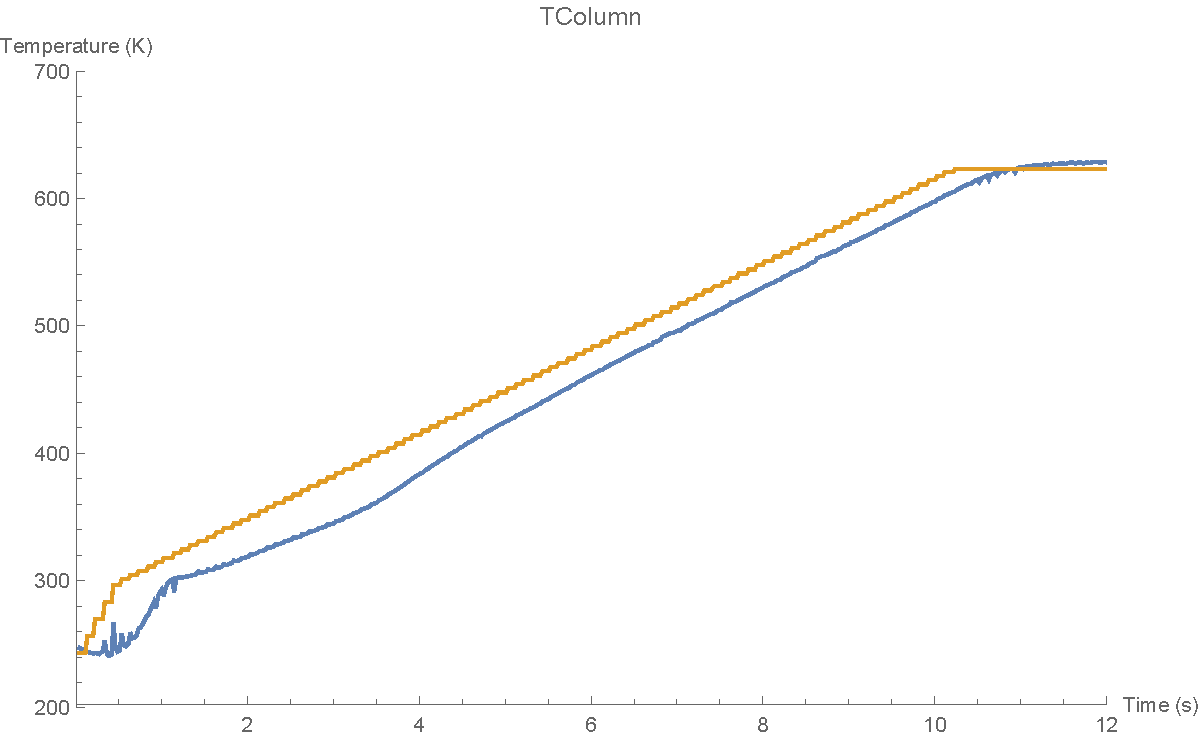
\includegraphics[width=\textwidth]{Figures/Setpoint_Following.pdf}
	\decoRule	
	
\caption[The fidelity of a fast GC temperature program]{ The graph shows how
well the indicated temperature followed the fast temperature program. The orange
line shows the intended temperature program and the blue line shows the actual
indicated temperature, as recorded. The ``steps'' in the orange line is caused
by the \SI{100}{\milli\second} period of the control loop.}

	\label{fig:Setpoint_Following} 
\end{figure}

The detector was an FID at \SI{350}{\celsius}. The FID response was recorded as
fast GC chromatograms and the collected GC chromatograms were used to compile
the 2D chromatogram.

\section{Results}

Figure \ref{fig:PAH_FAMEs} shows the SFC×GC chromatogram of the diesel/biodiesel blend.

\begin{figure}
	\centering
	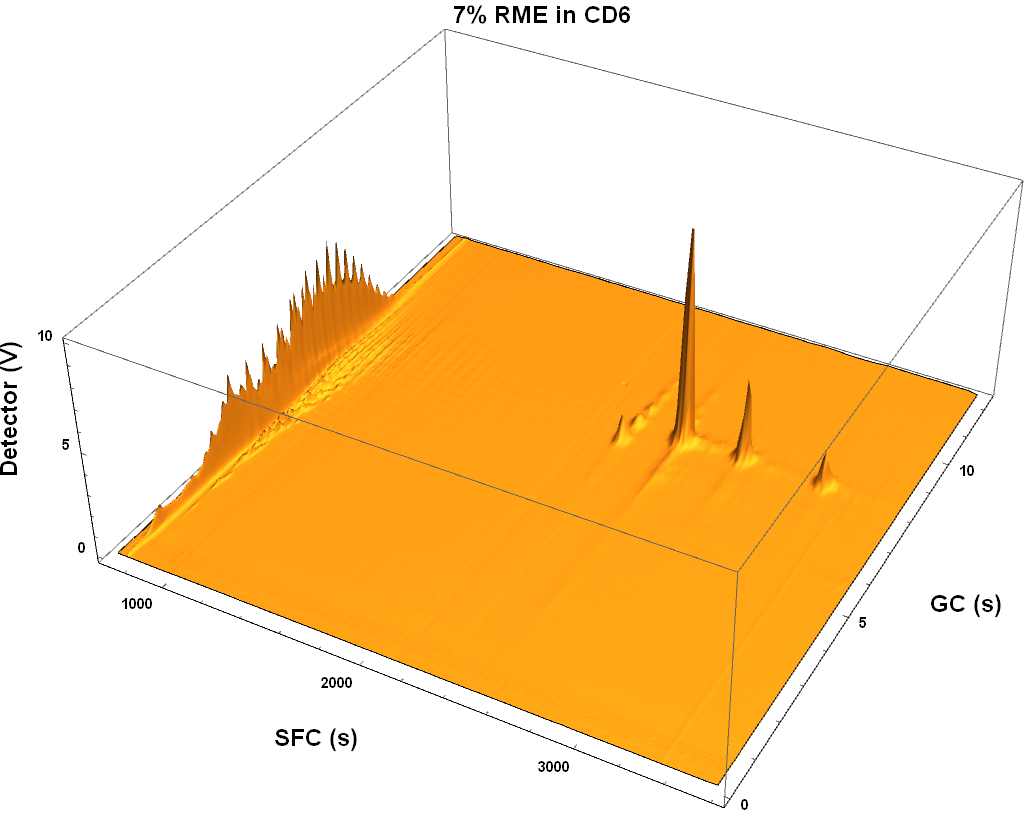
\includegraphics[width=\textwidth]{Figures/PAH_FAMEs.png}
	\decoRule	
	
\caption[Biodiesel separated from petrodiesel.]{A 2D chromatogram of the
biodiesel and petrodiesel in a \SI{7}{\percent} blend. The hydrocarbons elute
completely before the first FAME elute, offer interference-free determination of
both. The chromatogram was compiled from \num{368} 1D fast temperature-programmed GC
chromatogram}

	\label{fig:PAH_FAMEs} 
\end{figure}

Figure \ref{fig:Spiked_Diesel} shows the chromatogram of the diesel sample spiked with a selection of aromatic compounds. 

\begin{figure}
	\centering
	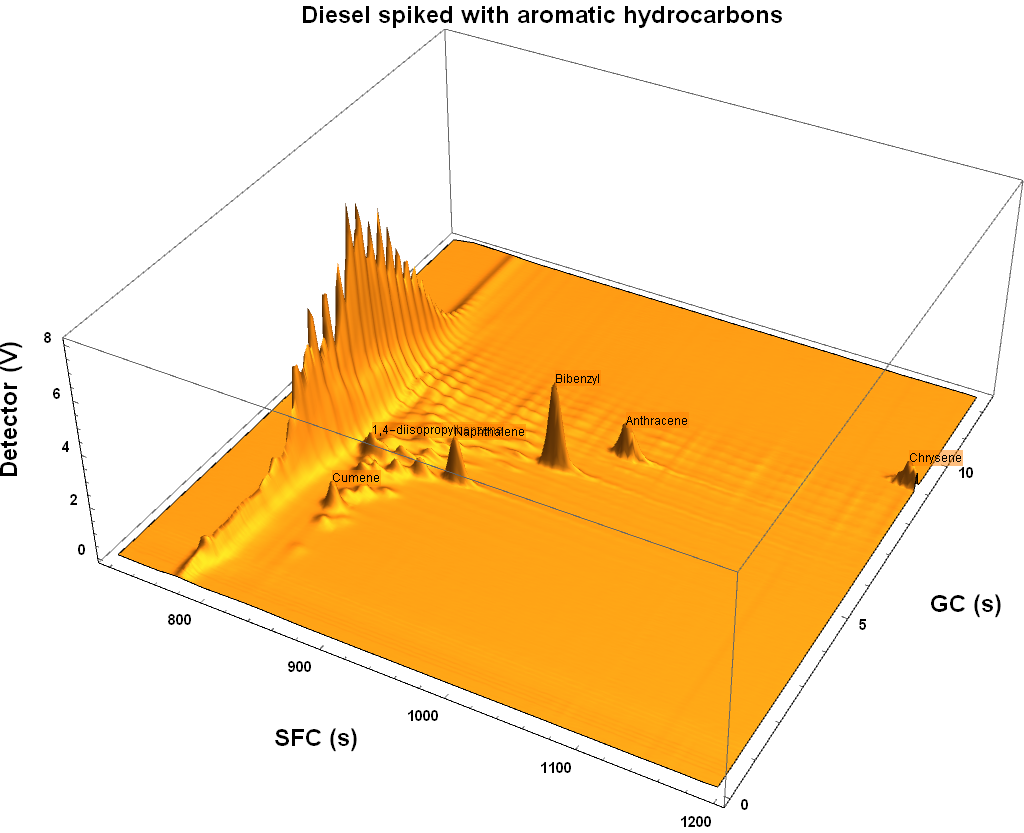
\includegraphics[width=\textwidth]{Figures/Spiked_Diesel.png}
	\decoRule	
	
\caption[Spiked diesel ]{A 2D chromatogram of a commercial diesel sample spiked with selected aromatic compounds.}

	\label{fig:Spiked_Diesel} 
\end{figure}


\section{Discussion}


The chromatogram of the biodiesel/petrodiesel blend (Figure \ref{fig:PAH_FAMEs}) shows
that the blend was separated into two distinct groups of compounds. At a \oneD
(SFC) retention time of about \SI{980}{\second} the hydrocarbons from the
petrodiesel part of the blend elute. To those familiar with petrochemical
chromatography the characteristic unresolved complex mixture (``hydrocarbon
hump'') topped by alkane peaks will be instantly recognizable as representing
a petroleum product. (See Figure \ref{fig:HCHump} for an example.)

\begin{figure}
	\centering
	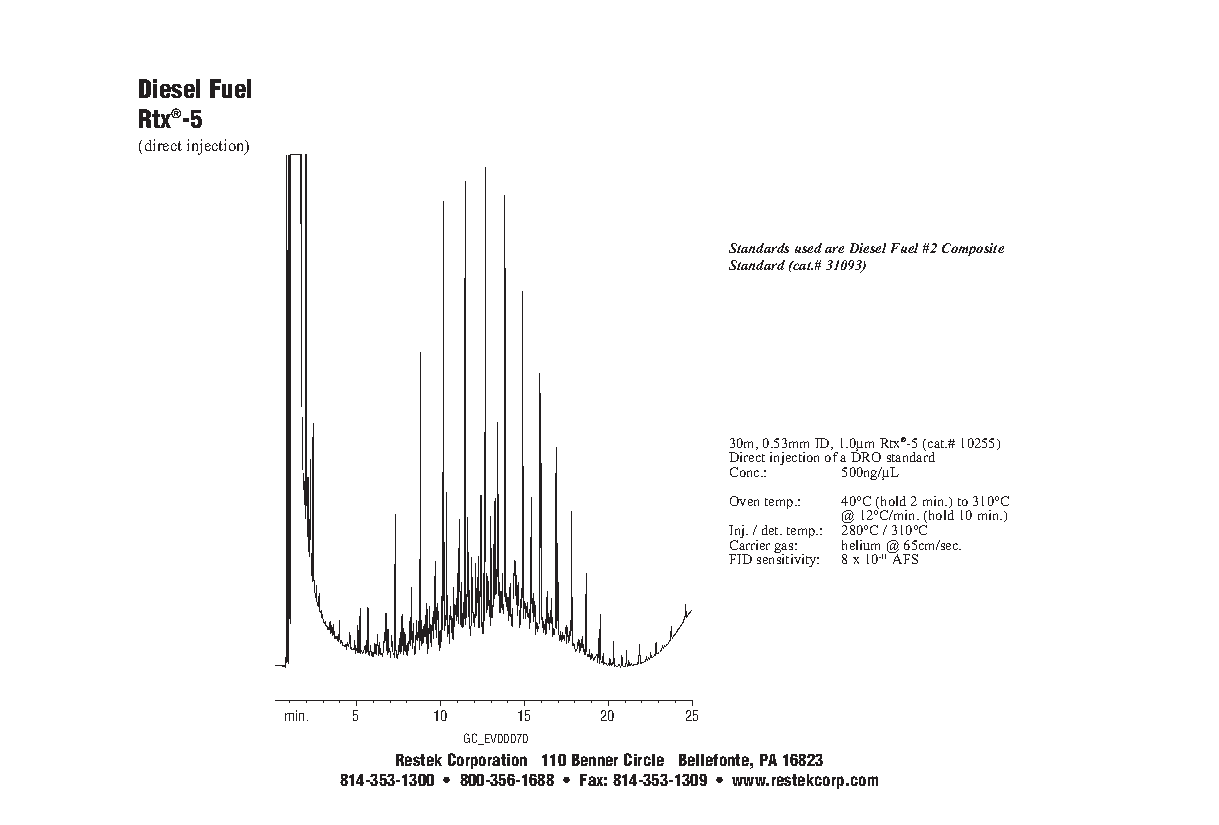
\includegraphics[width=\textwidth]{Figures/hchump.pdf}
	\decoRule	
	
\caption[An example of a petrochemical fuel chromatogram.]{An example of a GC
chromatogram obtained from a petroleum-based diesel fuel sample, showing the
unresolved complex mixture topped by alkane peaks.}
	
	\label{fig:HCHump} 
\end{figure}

At \(^{1}t_{r} \geq \) \SI{2200}{\second} a series of tall peaks represent the
FAMEs, in a pattern that was described in Chapter \ref{Chapter6}: \oneD
separation is according to the number of double bonds of the fatty acids, and
\twoD separation is according to the chain length of the fatty acids.


\subsection{Aromatic hydrocarbons}

Between \SI{980}{\second} and \SI{1200}{\second} a pattern of small peaks elute.
This portion of the chromatogram is shown magnified in Figure
\ref{fig:Hydrocarbons_Portion}, where individual peaks can clearly be distinguished.

\begin{figure}
	\centering
	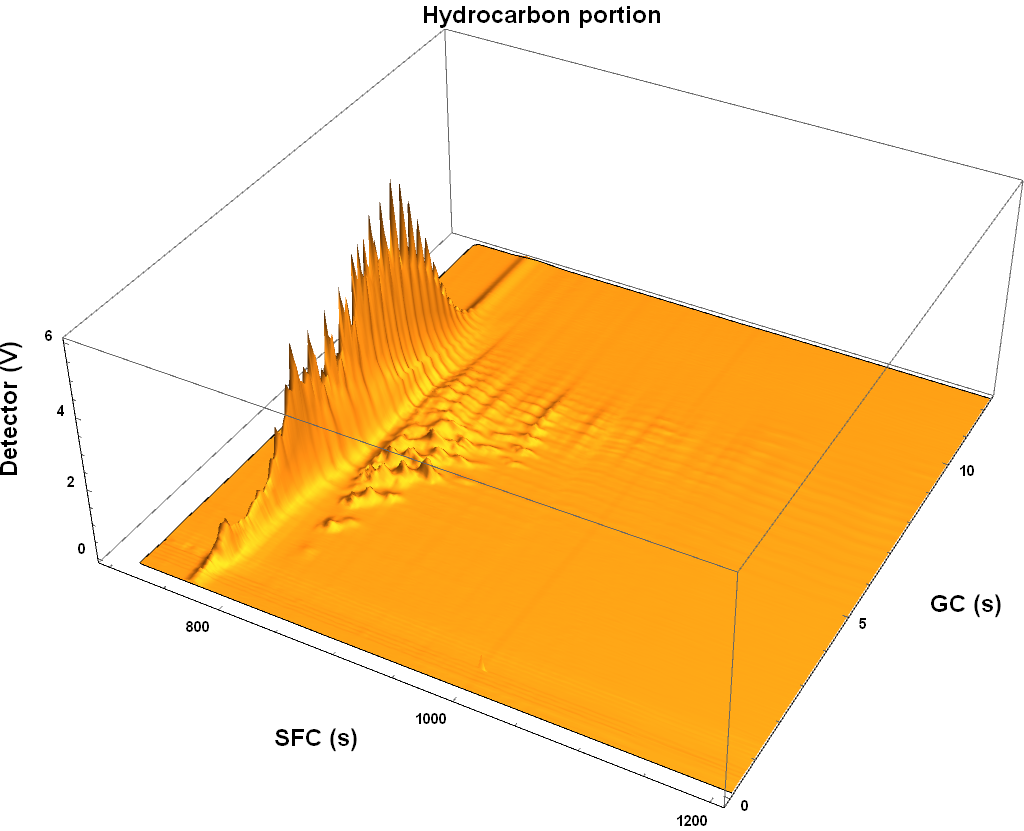
\includegraphics[width=\textwidth]{Figures/Hydrocarbons_Portion.png}
	\decoRule	
	
\caption[Hydrocarbons in RME/CD6 blend.]{Hydrocarbons in RME/CD6 blend}
	
	\label{fig:Hydrocarbons_Portion} 
\end{figure}

This result can be compared to the results of the SFC-FID method by integrating
each \twoD GC chromatogram, and plotting these values against their start times.
This creates a virtual SFC chromatogram, which should look similar to 1D SFC
chromatograms. The virtual SFC chromatogram corresponding to Figure
\ref{fig:Hydrocarbons_Portion} is shown in Figure \ref{fig:Virtual_SFC},
compared to an SFC-GC chromatogram taken from the paper on which ASTM 5186 is
based \autocite{DiSanzo1991}. The similarity between the virtual and real
chromatograms confirms that the pattern of peaks that elute shortly after the
alkanes are the aromatic hydrocarbons. The virtual chromatogram seems to show
that there is incomplete separation between the alkanes and the aromatics, but
the 2D chromatogram shows that there is complete separation. 

\begin{figure}
	\centering
	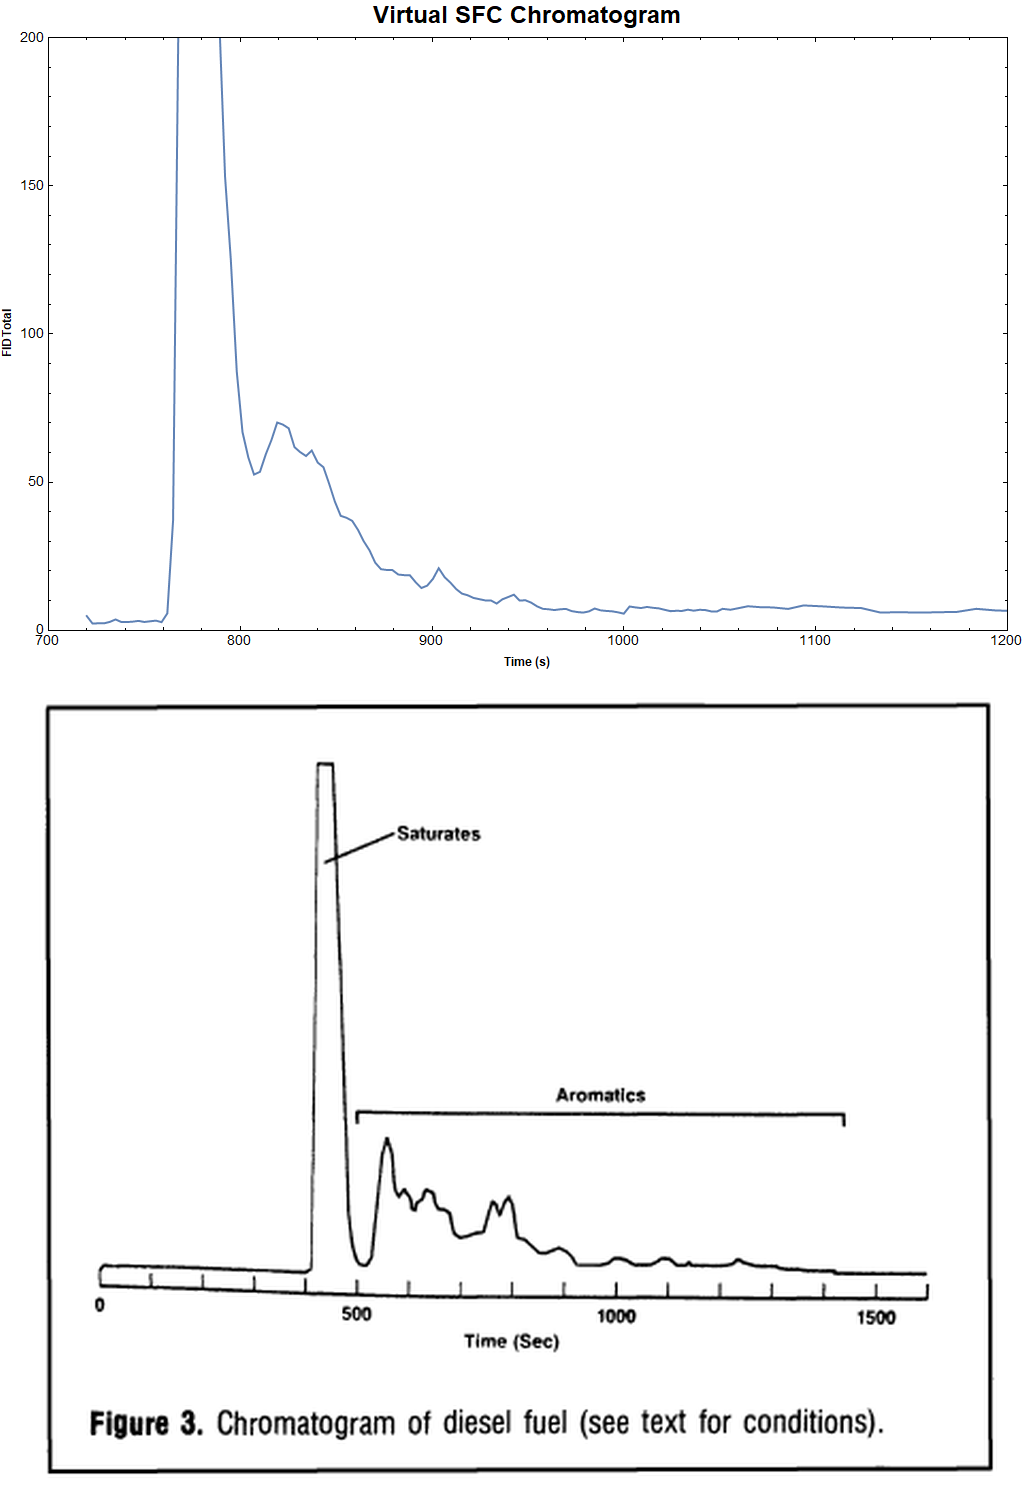
\includegraphics[width=\textwidth]{Figures/VirtualSFC_Compared.png}
	\decoRule	
	
\caption[Comparing SFC-FID and virtual SFC.]{Comparing SFC-FID and virtual SFC chromatograms.}
	
	\label{fig:Virtual_SFC} 
\end{figure}

Although the identification of peaks of aromatic hydrocarbons in the SFC×GC
chromatogram is beyond the scope of this project, injection of the spiked diesel
sample confirms that aromatic compounds elute in this region and shows that the
PAHs in diesel can be clearly separated from the alkanes and quantified. By
comparing the boiling points and relative masses of the spike compounds, a
tentative peak assignment could be made, as shown in Figure
\ref{fig:Spiked_Diesel_Annotated}.

\begin{figure}
	\centering
	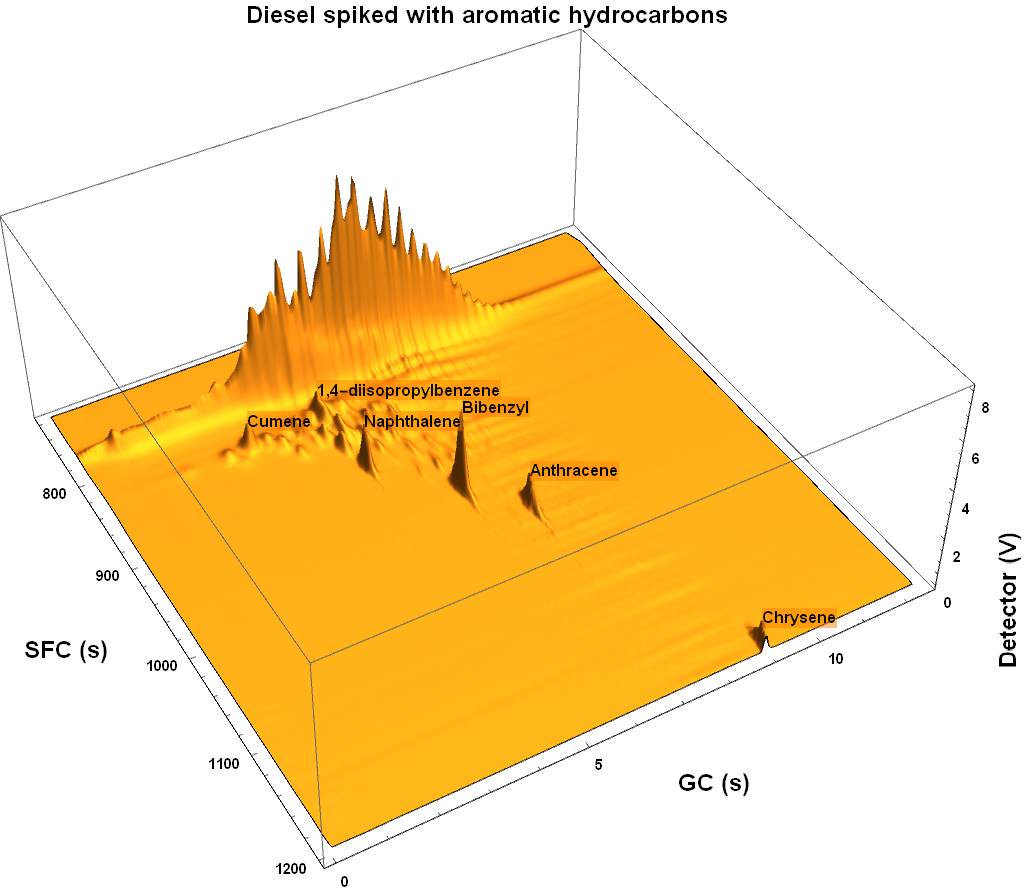
\includegraphics[width=\textwidth]{Figures/Spiked_Diesel_Annotated.png}
	\decoRule	
	
\caption[Peak assignment in spiked diesel sample.]{A 2D chromatogram of a
commercial diesel sample spiked with selected aromatic compounds. Tentative peak
assignments were made using knowledge of the boiling points and relative masses
of the spike compounds.}

	\label{fig:Spiked_Diesel_Annotated} 
\end{figure}

It should be noted that the 5-ring PAH benzo[a]pyrene that was spiked in did not
elute on this chromatogram. Its retention time is still unknown, but broad
interfering peaks have been recorded in subsequent chromatograms which can be
attributed to slowly-eluting benzo[a]pyrene. 

Previous work has shown that it is possible to also separate the alkenes from
the alkanes \autocite{Venter1999}, at least in petrol, and that the resolution
can be improved by cooling the SFC column. Further research along these lines
might reveal that is possible to separate the alkenes from the alkanes in
diesel. While cooling requires more hardware, the SFC×GC discussed in this
thesis offers two sources of cooling that might be exploited in such a project:
a portion of the coolant used to cool the SFC pump and the cryogen reservoir can
be diverted to cool the column, or any excess coolant from the
cooling cycle of the fast GC can be used to also cool the SFC column.
Alternatively, small solid-state Peltier cooling devices used for cooling
integrated circuits are readily available on the consumer market.

\subsection{FAMEs}

Between the \textsuperscript{1}D retention times of \SI{2200}{\second} and
\SI{3200}{\second} the peaks of the FAMEs are seen, clearly separated by number
of double bonds in the SFC dimension, and by volatility in the GC dimension.
When compared to Figure \ref{fig:2DCanola}, the pattern is clearly similar, so
the label ``rapeseed methyl ester'' is not incorrect.

\subsection{Adjustable modulation}

Because the SFC is operated in stopped flow mode, the modulation period is
independent of the fast GC run times. This means that the modulation period can
be adapted during the SFC×GC chromatographic run. Short modulation periods might
be required to preserve resolution obtained in the \oneD separation but this
will increase the total SFC×GC run time. In areas of the chromatogram where
there is plenty of resolution the modulation period might be increased to
decrease the run time.

In the chromatogram of the biodiesel blend (Figure \ref{PAH_FAMEs}), the modulation period was
\SI{3}{\second} up to a \oneD retention time of \SI{1100}{s}. After that the
modulation period was increased to \SI{10}{\second}, which shortened the
chromatographic run time. In this instrument this is the upper limit of the
modulation period, and is determined by the flow of carbon dioxide that the FID
flame can tolerate. If the flow of carbon dioxide through the column during
trapping becomes too high, the flame is extinguished and the signal disappears.
This limitation can fairly simply be overcome by arranging automatic re-ignition
of the flame. Then the upper limit of the modulation period depends on the
pressure limits of the GC inlet. These might be mechanical, but experience has
also taught that overly high inlet pressures can damage pressure gauges without
any other sign of over-pressure.

\subsubsection{Trapping suspension}

In an extreme version of adjustable modulation, it is also possible  suspend
trapping. This is implemented by opening both the SFC stop valve and the GC
inlet vent. The SFC elaute is then swept out of the GC inlet with no, or
mininal, trapping on the GC column. This scheme might be used, for example,
between \(^{1}t_r = 1200\) and \(^{1}t_r = 2200\) during the diesel blend
chromatogram. No peaks of interest elute during this period, so suspending
trapping can save a lot of time.

\subsubsection{Variable temperature programs}

Because stop-flow operation decouples the SFC and the GC, the modulation period
is independent of the GC run time as discussed in the previous sections. But
this also implies that, conversely,  the GC run time is independent of the
modulation period. This means that the GC fast temperature program can be
adapted to suit the GC separation of the different classes of compounds
as separated by the SFC.

\subsection{Application}

This separation shows that SFC×GC can be used to investigate the amount FAMEs and PAHs
petrodiesel/biodiesel blends without sample pre-treatment or
specialized columns. The intrinsic orthogonality provides easy identification of
components and the excess separation space allows for the addition of suitable
internal standards for reliable qualitative and quantitative analysis with the
robust FID with its predictable response. Expensive mass spectrometric detection
is unnecessary.

Being able to determine the biodiesel content of biodiesel blends may prove
useful in at least two scenarios: 

The first is in monitoring blending. Biodiesel (essentially a mixture of esters)
is quite polar compared to petrodiesel (essentially a mixture of hydrocarbons).
This means that blending might not be a matter of just pumping the relevant volumes
of the respective fuels into a tank and relying on diffusion to complete the
mixing. Being able to determine the amount of biodiesel in different samples of
a blend will provide assurance that the blend is homogenous and should perform
according to expectations. While such a test is perhaps better performed using a
spectroscopic method, SFC×GC can provide information for calibration, and will
of course be invaluable during trouble shooting.  

The second application of SFC×GC is in regulating diesel content. In some
political environments fuels might be taxed according to their
biologically-derived content, for example to promote agriculture or to meet
carbon emissions targets. Sometimes biological content is not encouraged by
taxation, but simply mandated. Such incentives and mandates are of course liable
to corruption, and therefore the ability to monitor the blending of the fuels is
needed. The most reliable way to differentiate between organic matter derived
from biological sources and organic matter derived from fossil sources is a
radiochemical method, where the content of radioactive \textsuperscript{14}C is
determined. (Organic material from fossil sources contains no
\textsuperscript{14}C.) The technical standard ASTM D6866 provides an approved
method. But radiochemical methods require specialized equipment and trained
staff, whereas fuel laboratories more often have experience with chromatographic
techniques and might find SFC×GC a useful technique to provide evidence that a
diesel fuel blend contains the stated amount of biodiesel.
\begin{todo}Virtual SFC\end{todo}

\section{Conclusion}


, and might provide a way to quantify the biodiesel component in blends
with petrodiesel, and cost-effective, accurate and reliable quantitation of the
biodiesel component in blends with petrodiesel can be expected.



\todos